\subsection{Оптические атмосферные эффекты}

В этом разделе будут рассмотрены известные оптические эффекты, возникающие в атмосфере Земли. Их можно разделить на три группы по природе происхождения. Так, \term{радуга} (см.~\ref{sec:rainbow}) формируется в ходе рефракции и отражения света в достаточно крупных каплях воды, распыленных в воздухе. Различные виды \term{гало} (см.~\ref{sec:halo})~--- \imp{$\mathit{22^\circ}$ гало}, \imp{зенитная дуга}, \imp{округло-горизонтальная дуга} и \imp{паргелий}, формируются в результате прохождения света через кристаллы льда, находящиеся в воздухе. А такие эффекты как \imp{глория}, \imp{венец (корона)} и \imp{радужные облака} формируются в ходе  диффракции света на мелких каплях или кристаллах льда, или других частицах, например, частицы дыма или мелкий песок.\,\cite{atmospheric-optics}

\subsubsection{Радуга}
\label{sec:rainbow}

\newcommand{\drawRainbow}[2][1]{
    \tkzInit[xmin=-0.4, ymin=-1.5*#1, xmax=2.1, ymax=1.1*#1]
    \tkzClip
    
    \tkzDefPoint(0,0){R}
    \tkzDefPoint(1,0){C}
    
    \foreach \x in {-0.02,-0.04,...,-1} {
%        \tkzSetUpLine[gray]

        \tkzDefPoint(-0.5,\x){A}
        \tkzDefPoint(0,\x){B}
        
        \tkzInterLC(B,A)(C,R) 
        \tkzGetPoints{R1}{x}
        
        \tkzDrawSegment[gray](A,R1)
        
        \tkzFindAngle(A,R1,C) 
        \tkzGetAngle{ABC}
        
        \pgfmathparse{\ABC - 180}
        \pgfmathsetmacro\ALPHA{\pgfmathresult}
        
        \pgfmathparse{asin(sin(\ALPHA)/1.333)}
        \pgfmathsetmacro\BETA{\pgfmathresult}
        
        \tkzDefPointBy[homothety=center R1 ratio 1](R1) 
        \tkzGetPoint{R2}
        \foreach \i in {0,1,...,#2} {
            \tkzDefPointBy[rotation=center R1 angle -\BETA](C) 
            \tkzGetPoint{R1'}
            
            \tkzInterLC(R1,R1')(C,R) 
            \tkzGetPoints{x}{R2}
            
            \tkzDrawSegment[gray](R1,R2)
            
            \tkzDefPointBy[homothety=center R1 ratio 1](R2) 
            \tkzGetPoint{R1}
        }
        
        \tkzDefPointBy[rotation=center R1 angle -180 + \ALPHA](C) 
        \tkzGetPoint{L'}
        
        \tkzDefPointBy[homothety=center R1 ratio 1.5](L') 
        \tkzGetPoint{L}
        
        \tkzDrawSegment[gray](R2,L)
    }
        
    \tkzDefPoint(-0.5,0){A0}
    \tkzDefPoint(2,0){B0}
    \tkzDrawSegment[dotted, thick](A0,B0))
        
    \tkzDrawCircle[thick, black](C,R)
}
\def\drawRainbowDispersion(#1){% (count)
    \tkzInit[xmin=-0.4, ymin=-1.5, xmax=2.1, ymax=1.1]
    \tkzClip
    
    \tkzDefPoint(0,0){R}
    \tkzDefPoint(1,0){C}
    
    \foreach \n in {1.332,1.334,...,1.345} {
        \tkzSetUpLine[gray]

        \pgfmathparse{sqrt((1 + #1)^2 -\n^2)/sqrt(2 * #1 + #1 * #1)}
        \pgfmathsetmacro\x{\pgfmathresult}

    
        \tkzDefPoint(-0.5,-\x){A}
        \tkzDefPoint(0,-\x){B}
        
        \tkzInterLC(B,A)(C,R) 
        \tkzGetPoints{R1}{x}
        
        \tkzDrawSegment(A,R1)
        
        \tkzFindAngle(A,R1,C) 
        \tkzGetAngle{abc}
        
        \pgfmathparse{\abc - 180}
        \pgfmathsetmacro\ALPHA{\pgfmathresult}
            
        \pgfmathparse{asin(sin(\ALPHA)/\n)}
        \pgfmathsetmacro\BETA{\pgfmathresult}
        
        \tkzDefPointBy[homothety=center R1 ratio 1](R1)
        \tkzGetPoint{R2}
        
        \foreach \i in {0,1,...,#1} {
            \tkzDefPointBy[rotation=center R1 angle -\BETA](C) 
            \tkzGetPoint{R1'}
            
            \tkzInterLC(R1,R1')(C,R) 
            \tkzGetPoints{x}{R2}
            
            \tkzDrawSegment(R1,R2)
            
            \tkzDefPointBy[homothety=center R1 ratio 1](R2) 
            \tkzGetPoint{R1}
        }
                
        \pgfmathparse{-180+\ALPHA}
        \pgfmathsetmacro\r{\pgfmathresult}
        
        \tkzDefPointBy[rotation=center R1 angle \r](C) 
        \tkzGetPoint{L'}
        
        \tkzDefPointBy[homothety=center R1 ratio 1](L') 
        \tkzGetPoint{L}
        
        \tkzDrawSegment(R1,L)
    }
        
    \tkzDefPoint(-0.5,0){A0}
    \tkzDefPoint(2,0){B0}
    \tkzDrawSegment[dotted, thick](A0,B0))
        
    \tkzDrawCircle[thick, black](C,R)
}

Радуга~--- событие проявления преломления (рефракции) и отражения солнечного света, в каплях воды, распыленных в воздуха. Наблюдается в виде ярких разноцветных колец, перпендикулярных прямой \textsl{Солце -- наблюдатель}, с центром на ней. 

Стоит обратить внимание на возможность обобщения данной формулировки. Излучение может быть монохромным, тогда радуга будет также монохромна. Для появления радуги необязательно наличие воздуха. Данного эффекта можно достичь, распыляя воду в космосе~--- без атмосферы и гравитации. Также радуга может наблюдаться во взвеси стеклянных шариков или капель любой другой прозрачной для рассматриваемого излучения жидкости.

Рассмотрим детальнее, как формируются радужные кольца. Для упрощения расчетов солнечный свет можно считать параллельным фронтом с выделенным направлением, а капли воды с достаточной точностью сферическими. 

\begin{wrapfigure}[13]{r}{0.47\tw}
    \vspace{-1.5pc}
    \tikzsetnextfilename{rainbow-scheme}
\begin{tikzpicture}[
    scale=2,
    arrow/.style 2 args={
        postaction=decorate,
        decoration={
            markings, 
            mark=at position #2 with {\arrow{#1}}
        } 
    }
]
    \tkzInit[xmin=-0.55, ymin=-1.2, xmax=2.15, ymax=1.15]
    \tkzClip
    
    \tkzDefPoint(0,0){R}
    \tkzDefPoint(1,0){C}

    \tkzDefPoint(-0.5,0.8){A}
    \tkzDefPoint(0,0.8){B}
    
    \tkzInterLC(B,A)(C,R) 
    \tkzGetPoints{x}{R1}
    
    \tkzFindAngle(A,R1,C) 
    \tkzGetAngle{ABC}
    
    \pgfmathparse{180 - \ABC}
    \pgfmathsetmacro\ALPHA{\pgfmathresult}
    
    \pgfmathparse{asin(sin(\ALPHA)/1.333)}
    \pgfmathsetmacro\BETA{\pgfmathresult}
    
    \tkzDefPointBy[rotation=center R1 angle \BETA](C) 
    \tkzGetPoint{R1'}
    \tkzInterLC(R1,R1')(C,R) 
    \tkzGetPoints{R2}{x}
    
    \tkzDefPointBy[rotation=center R2 angle \BETA](C) 
    \tkzGetPoint{R2'}
    \tkzInterLC(R2,R2')(C,R) 
    \tkzGetPoints{R3}{x}
    
    \tkzDefPointBy[rotation=center R3 angle \BETA](C) 
    \tkzGetPoint{R3'}
    \tkzInterLC(R3,R3')(C,R) 
    \tkzGetPoints{R4}{x}
    
    \tkzDefPointBy[rotation=center R4 angle 180-\ALPHA](C) 
    \tkzGetPoint{L}
    
    \tkzDefPoint(-0.5,0){A0}
    \tkzDefPoint(2,0){B0}
    \tkzDrawSegment[dash dot, thick](A0,B0)
%    
    \tkzDrawSegments[arrow={latex}{0.5}](R1,R2 R2,R3 R3,R4 R4,L)
    \tkzDrawSegments[arrow={latex}{0.7}](A,R1)
    \tkzDrawLines[dashed](C,R2 C,R3)
    
    \tkzMarkAngle[line width = 0.15pt, size=0.01](C,R1,R2) % костыль для расстояния между дугами
    \tkzMarkAngles[size = 0.25](C,R1,R2 C,R2,R3 C,R3,R4)
    \tkzMarkAngles[size = 0.3](R1,R2,C R2,R3,C R3,R4,C)
    \tkzLabelAngles[pos=0.4, fill=white, inner sep=1pt](C,R1,R2 C,R2,R3 C,R3,R4 R1,R2,C R2,R3,C R3,R4,C){\footnotesize $\beta$}
    
    
    \tkzDefPointBy[homothety=center R1 ratio -0.5](C) \tkzGetPoint{C1}
    \tkzDefPointBy[homothety=center R2 ratio -0.5](C) \tkzGetPoint{C2}
    \tkzDefPointBy[homothety=center R3 ratio -0.5](C) \tkzGetPoint{C3}
    \tkzDefPointBy[homothety=center R4 ratio -.15](C) \tkzGetPoint{C4}
    
    \tkzDrawLines[dashed](C,C1 C,C4)
    \tkzMarkAngles[size=0.15, arc=ll](C1,R1,A L,R4,C4)
    \tkzLabelAngles[pos=0.3,font=\footnotesize](C1,R1,A L,R4,C4){$\alpha$}
    
    \tkzDefPointBy[rotation=center R1 angle -90](C) \tkzGetPoint{T1}
    \tkzDefPointBy[rotation=center R2 angle  90](C) \tkzGetPoint{T2}
    \tkzDefPointBy[rotation=center R3 angle  90](C) \tkzGetPoint{T3}
    \tkzDefPointBy[rotation=center R4 angle  90](C) \tkzGetPoint{T4}
    
    
    \tkzMarkRightAngles[size=0.1](T1,R1,C T2,R2,C2 T3,R3,C3 C,R4,T4)
    
    \tkzInterLL(R4,L)(A,R1)
    \tkzGetPoint{W}
    \tkzMarkAngle[line width = 0.2pt, size=0.01](C,R1,R2) % костыль для расстояния между дугами
    \tkzMarkAngle[arc=lll, size=0.15](R1,W,L)
    \tkzLabelAngle[pos=0.3, font=\footnotesize](R1,W,L){$\omega$}
    
    \tkzDefMidPoint(A,R1)  \tkzGetPoint{M0}
    \tkzDefMidPoint(R1,R2) \tkzGetPoint{M1}
    \tkzDefMidPoint(R2,R3) \tkzGetPoint{M2}
    \tkzDefMidPoint(R3,R4) \tkzGetPoint{M3}
    \tkzDefMidPoint(R4,L)  \tkzGetPoint{M4}
    
    \tkzDefPointBy[homothety=center A ratio 0.1](R1) \tkzGetPoint{A'}
    \tkzDefPointBy[translation=from A to A'](A0)    \tkzGetPoint{A0'}
    \tkzDrawSegment[latex-latex](A',A0')
    \tkzLabelSegment[left, font=\footnotesize](A',A0'){$\rho$}
    
    \tkzDrawCircle[thick, black](C,R)
    
    \tkzDrawPoints(C, R1, R2, R3, R4)
\end{tikzpicture}

    \caption{Схема следования луча в капле при $k=2$}
\end{wrapfigure}
Представим такую каплю и отметим выделенное направление падения света пунктиром (см.~Рис.\,\ref{pic:rainbow}). Рассмотрим луч, падающий на каплю на расстоянии $\rho \in [0,1]$ радиусов капли от её оси. В таком случае угол падения луча на поверхность капли $\alpha = \arcsin \rho$. Пусть $n$~--- коэффициент преломления воды, тогда по закону Снеллиуса угол преломления 
\begin{equation*}
    \beta = \arcsin \frac{\sin{\alpha}}{n} = \arcsin \frac{\rho}{n}.
\end{equation*}
Так как $\beta$~--- угол между радиусом и преломленным лучем, то преломленный луч вновь пересечется с поверхностью капли на угловом расстоянии $180^\circ - 2\beta$ в сторону движения луча. 

В точке пересечения преломленного луча с поверхностью капли часть света преломится и выйдет наружу, а остальная часть отразится от внутренней поверхности под углом $\beta$ согласно закону отражения. И~на угловом расстоянии $180^\circ - 2\beta$ вновь частично преломится и покинет каплю, а частично отразится и продолжит свой путь внутри капли.

Определим \imp{порядок} радуги $k$ как число отражений луча от внутренней поверхности капли. Тогда при формировании радуги $k$-ого порядка луч света, проходящий на расстоянии $\rho$ радиусов капли от её оси с точностью до целого числа полных оборотов поворачивается на угол 
\begin{multline*}
    \omega 
        = 2(\alpha - \beta) + k (\pi - 2\beta) 
        = 2\alpha - 2\beta(k + 1) + \pi (k \!\!\!\! \mod 2) = \\
        = 2\arcsin \rho - 2(k + 1) \arcsin \frac{\rho}{n} + \pi (k \!\!\!\!  \mod 2). 
\end{multline*}

Радуга выделяется на фоне за счет своей яркости, которая достигается из-за увеличения плотности потока излучения, выходящего из капли после $k$ отражения, в конкретном направлении. Что соответствует равенству нулю производной $\partial\omega/\partial\rho$. Определим значение~$\rho$, при котором это происходит, чтобы найти угловой радиус радуги $k$-ого порядка.
\begin{gather*}
    \frac{\partial \omega}{\partial \rho} = \frac{2}{\sqrt{1 - \rho^2}} - \frac{k + 1}{\sqrt{n^2 - \rho^2}} = 0,\quad \rho \in [0,1];\\
%    \sqrt{n^2 - \rho^2} - (k + 1) \sqrt{1 - \rho^2} = 0,\quad \rho \in [0,1);\\
%    n^2 - \rho^2 = (k+1)^2(1 - \rho^2), \quad \rho \in [0,1) ;\\
    \rho = \sqrt{\frac{(k+1)^2 - n^2}{(k+1)^2 - 1}},\quad \rho \in [0, 1).
\end{gather*}

Коэффициент преломления воды в оптическом диапазоне зависит от длины волны практически линейно, принимая значения от $n_\text{к} = 1.331$ для красного света ($\lambda = 700$~нм) до $n_\text{ф} = 1.344$ для фиолетового ($\lambda = 400$~нм). Таким образом внешний край \imp{первичной} радуги имеет радиус~$42.4^\circ$ и красный цвет, а внутренний~---~$40.5^\circ$ и фиолетовый цвет,  \lookPicRef{pic:rainbow-disp-1}.
\imp{Вторичная} радуга имеет размер от~$50.4^\circ$ для красного до~$53.7^\circ$ для фиолетового, \lookPicRef{pic:rainbow-disp-2}. Важно отметить, из-за дополнительного отражения цвета вторичной радуги идут в обратном порядке относительно первичной. 

\begin{figure}[t]
    \begin{subcaptionblock}{0.3\tw}
        \centering
        \tikzsetnextfilename{rainbow-1-scheme}
        \begin{tikzpicture}[scale=1.3]
            \begin{scope}[yscale=-1]
                \drawRainbow[-1]{1}
            \end{scope}
        \end{tikzpicture}
        \caption{$k=1$}
        \label{pic:rainbow-1}
    \end{subcaptionblock}
    \hfill
    \begin{subcaptionblock}{0.3\tw}
        \centering
        \tikzsetnextfilename{rainbow-2-scheme}
        \begin{tikzpicture}[scale=1.3]
            \drawRainbow{2}
        \end{tikzpicture}
        \caption{$k=2$}
        \label{pic:rainbow-2}
    \end{subcaptionblock}
    \hfill
    \begin{subcaptionblock}{0.3\tw}   
        \centering
        \tikzsetnextfilename{rainbow-3-scheme}
        \begin{tikzpicture}[scale=1.3]
            \drawRainbow{3}
        \end{tikzpicture}
        \caption{$k=3$}
        \label{pic:rainbow-3}
    \end{subcaptionblock}
    \caption{Схема хода лучей при формировании радуги $k$-ого порядка}
    \label{pic:rainbow}
\end{figure}
\begin{figure}[h!]
    \begin{subcaptionblock}{0.3\tw}
        \centering
        \tikzsetnextfilename{rainbow-1-dispersion}
        \begin{tikzpicture}[scale=1.3]
            \begin{scope}[yscale=-1]
                \drawRainbowDispersion[-1]{1}
            \end{scope}
            \tkzDefPoint(1.2,-1.15){Label}
            \tkzLabelPoint[below=-1pt](Label){\tiny$42.4^\circ$}
            \tkzLabelPoint[left=6pt](Label){\tiny$40.5^\circ$}
        \end{tikzpicture}
        \caption{$k=1$}
        \label{pic:rainbow-disp-1}
    \end{subcaptionblock}
    \hfill
    \begin{subcaptionblock}{0.3\tw}
        \centering
        \tikzsetnextfilename{rainbow-2-dispersion}
        \begin{tikzpicture}[scale=1.3]
            \begin{scope}
                \drawRainbowDispersion{2}
            \end{scope}
            \tkzDefPoint(-0.2,-0.3){Label}
            \tkzLabelPoint[below](Label){\adjustbox{right=18pt, raise=12pt}{\tiny$53.7^\circ$}}
            \tkzLabelPoint[above](Label){\adjustbox{raise=18pt}{\tiny$50.4^\circ$}}
        \end{tikzpicture}
        \caption{$k=2$}
        \label{pic:rainbow-disp-2}
    \end{subcaptionblock}
    \hfill
    \begin{subcaptionblock}{0.3\tw}
        \centering
        \tikzsetnextfilename{rainbow-3-dispersion}
        \begin{tikzpicture}[scale=1.3]
            \drawRainbowDispersion{3}
            \tkzDefPoint(1.1,-1.3){Label}
            \tkzLabelPoint[above right=-2pt](Label){\tiny${37.7^\circ}$}
            \tkzLabelPoint[below left=-1pt](Label){\adjustbox{raise=15pt}{\tiny${42.5^\circ}$}}
        \end{tikzpicture}
        \caption{$k=3$}
        \label{pic:rainbow-disp-3}
    \end{subcaptionblock}
    \caption{Схема дисперсии лучей при формировании радуги $k$-ого порядка}
\end{figure}

Обе радуги, несложно заключить, расположены напротив Солнца и их радиус отсчитывается от противосолнечной точки. Отсюда следует важное замечание, чем ниже Солнце расположено над горизонтом, тем выше радуги первого и второго порядков. Напротив, \imp{третичная} радуга расположена со стороны Солнца на расстоянии от~$37.7^\circ$ для фиолетового до~$42.5^\circ$ для красного цветов, \lookPicRef{pic:rainbow-disp-3}.

В заключение необходимо объяснить применимость геометрической оптики в изложенных выше рассуждениях. Чаще всего радуга наблюдается до или после дождя, капли которого существенно больше капель тумана или облаков и достигают нескольких миллиметров в диаметре. Это больше характерной длины волны видимого глазом излучения на три--четыре порядка, что позволяет не учитывать волновые свойства света. В силу последних капли существенно меньшего размера могут вообще не сформировать радугу. 
\subsubsection{Гало}
\label{sec:halo}

Как было сказано выше, различные виды \imp{гало} наблюдаются в результате рефракции солнечного света в кристаллах льда, составляющих перистые облака. Эти облака в среднем находятся на высоте от 5 до 10~км, имеют температуру около $-40^\circ$C, почему состоят исключительно из кристаллов льда.


\begin{wrapfigure}[6]{r}{0.3\tw}
    \centering
    \vspace{-0.7pc}
    \newcommand{\drawPrizm}[2]{
        \tkzDefPoint(0,0){C}
        \def\R{#1}
        \def\h{#2}
        \def\f{0}

        \tkzDefShiftPoint[C](\R,0){x}
        \tkzDefPointBy[rotation=center C angle \f](x)  \tkzGetPoint{R1}
        \tkzDefPointBy[rotation=center C angle 60](R1) \tkzGetPoint{R2}
        \tkzDefPointBy[rotation=center C angle 60](R2) \tkzGetPoint{R3}
        \tkzDefPointBy[rotation=center C angle 60](R3) \tkzGetPoint{R4}
        \tkzDefPointBy[rotation=center C angle 60](R4) \tkzGetPoint{R5}
        \tkzDefPointBy[rotation=center C angle 60](R5) \tkzGetPoint{R6}

        \tkzGetPointCoord(R1){r}
        \tkzGetPointCoord(R2){R}
        \tkzGetPointCoord(R3){rr}
        \tkzGetPointCoord(R4){rR}
        \tkzGetPointCoord(R5){Rr}
        \tkzGetPointCoord(R6){RR}

        \draw[dashed] (\rx,\ry,0) -- (\Rx,\Ry,0) -- (\rrx,\rry,0) -- (\rRx,\rRy,0);
        \draw (\rRx,\rRy,0) -- (\Rrx,\Rry,0) -- (\RRx,\RRy,0) -- (\rx,\ry,0);

        \draw (\rx,\ry,\h) -- (\Rx,\Ry,\h) -- (\rrx,\rry,\h) -- (\rRx,\rRy,\h) -- (\Rrx,\Rry,\h) -- (\RRx,\RRy,\h) -- cycle;

        \draw (\rx,\ry,0) -- (\rx,\ry,\h);
        \draw[dashed] (\Rx,\Ry,0) -- (\Rx,\Ry,\h);
        \draw[dashed] (\rrx,\rry,0) -- (\rrx,\rry,\h);
        \draw (\rRx,\rRy,0) -- (\rRx,\rRy,\h);
        \draw (\Rrx,\Rry,0) -- (\Rrx,\Rry,\h);
        \draw (\RRx,\RRy,0) -- (\RRx,\RRy,\h);
    }

    \tikzsetnextfilename{column-cristal}
    \tdplotsetmaincoords{70}{165}
    \begin{tikzpicture}[tdplot_main_coords]
        \drawPrizm{0.4}{1.5}
    \end{tikzpicture}
    \tikzsetnextfilename{plate-cristal}
    \tdplotsetmaincoords{70}{185}
    \begin{tikzpicture}[tdplot_main_coords]
        \drawPrizm{0.9}{0.3}
    \end{tikzpicture}
    \caption{}
    \label{}
\end{wrapfigure}

В условия формирования перистых облаков кристаллы льда имеют шестиугольную симметрию и являются прямоугольными шестиугольными призмами. Их боковые грани могут иметь разные пропорции, но угол между соседними всегда составляет $60^\circ$. В дальнейшем будем разделять кристаллы на два вида: пластинчатые~--- размер оснований много больше высоты призмы, и колончатые~--- наоборот, высота призмы существенно больше размеров основания.~\cite{Champion_1981}

\paragraph{$\mathbf{22^\circ}$ гало}

\begin{wrapfigure}[11]{r}{0.25\tw}
    \vspace{-1pc}
    \centering
    \begin{tikzpicture}
    
	    \tkzDefPoint(0,0){C}
	    
	    \def\R{2}
	    \def\f{0}
	    \def\n{1.31}
	    
	    \tkzInit[
	       xmin={-0.2*\R},
	       xmax={1.1*\R},
	       ymin={-1.1*\R},
	       ymax={1.3*\R},
	    ]
	    \tkzClip
	    
	    
	    \tkzDefShiftPoint[C](\R,0){x}
	    \tkzDefPointBy[rotation=center C angle \f](x)  \tkzGetPoint{R1}
	    \tkzDefPointBy[rotation=center C angle 60](R1) \tkzGetPoint{R2}
	    \tkzDefPointBy[rotation=center C angle 60](R2) \tkzGetPoint{R3}
	    \tkzDefPointBy[rotation=center C angle 60](R3) \tkzGetPoint{R4}
	    \tkzDefPointBy[rotation=center C angle 60](R4) \tkzGetPoint{R5}
	    \tkzDefPointBy[rotation=center C angle 60](R5) \tkzGetPoint{R6}
	    
	    \tkzDrawPolygon[thick](R1,R2,R3,R4,R5,R6)
	    
	    \def\al{30}
	    \def\x{0.4}
	    
	    \tkzDefPointBy[homothety=center R2 ratio \x](R3) \tkzGetPoint{I}
	    \tkzDefLine[perpendicular=through I](R3,R2) \tkzGetPoint{I'}
	    
	    \def\bet{asin(sin(\al / 180 * pi) / \n)}
	    \def\b{\R * (sqrt(3) / 2  + (0.5 - \x) * tan(pi / 2 - \bet))}
	    \def\xo{(\b + sqrt(3) * \R) / (tan(pi / 2 - \bet) + sqrt(3))}
	    \def\yo{sqrt(3) * \xo - sqrt(3) * \R}
	    
	    \tkzDefPoint(\xo,\yo){O}
	    \tkzDefLine[perpendicular=through O](R1,R6) \tkzGetPoint{O'}
	    
	    \tkzInterLL(I,I')(O,O') \tkzGetPoint{T}
	    
	    \tkzDefPointBy[rotation=center I angle {-180 + \al}](T) \tkzGetPoint{x}
	    \tkzDefPointBy[homothety=center I ratio 0.4](x) \tkzGetPoint{A}
	    
	    \tkzFindAngle(I,O,T) \tkzGetAngle{gam}
	    \def\del{asin(\n * sin(\gam / 180 * pi)) * 180 / pi}
	    
	    \tkzDefPointBy[rotation=center O angle {180 - \del}](T) \tkzGetPoint{x}
	    \tkzDefPointBy[homothety=center O ratio 0.5](x) \tkzGetPoint{D}
	    
	    \tkzDrawSegment[arrow={latex}{0.3}](A,I)
	    \tkzDrawSegment[arrow={latex}{0.5}](I,O)
	    \tkzDrawSegment[arrow={latex}{0.9}](O,D)
	     
	    \tkzDrawLines[dashed, add=0.5cm and 0.5cm](I,T O,T)
	    
	    \tkzMarkRightAngles[size=0.2](R3,I,T T,O,R6)
	    
	    \tkzMarkAngle[arc=lll, size=0.5](T,I,O)
	    \tkzLabelAngle[pos=0.75](T,I,O){\footnotesize$\beta$}
	    
	    \tkzMarkAngle[arc=lll, mark=|, size=0.4, mksize=2](I',I,A)
	    \tkzLabelAngle[pos=0.6](I',I,A){\footnotesize$\alpha$}
	    
	    \tkzMarkAngle[line width = .3pt, size=0.01](I,O,T)
	    \tkzMarkAngle[arc=ll, size=0.3](I,O,T)
	    \tkzLabelAngle[pos=0.5](I,O,T){\footnotesize$\gamma$}
	    
	    \tkzMarkAngle[arc=ll, mark=|, size=0.3, mksize=2](D,O,O')
	    \tkzLabelAngle[pos=0.5](D,O,O'){\footnotesize$\delta$}
	    
	    \tkzMarkAngles[size=0.2](O,T,I R2,R1,R6 R3,R2,R1 R1,R6,R5)
	    \tkzLabelAngle[pos=0.5](O,T,I){\scriptsize$120^\circ$}
	   	    
	    \tkzDrawPoints(I, T, O, R1, R2, R6)
	\end{tikzpicture}
	\caption{}
	\label{}
\end{wrapfigure}
Яркая окружность вокруг Солнца, угловой радиус которой оставляет около $22^\circ$ в зависимости от длины волны излучения. Формируется в произвольно расположенных кристаллах в результате рефракции света на двух, следующих через одну, боковых гранях.

В зависимости от угла падения света на первую грань меняется угол итогового преломления, минимальная величина которого~--- примерно $22^\circ$. В силу экстремальности этого значения, наибольшее число кристаллов преломляют солнечный свет именно под этим углом.

Детально расмотрим геометрию формирования $22^\circ$~гало. Пусть~$\alpha$~--- угол падения луча на боковую грань $\mathcal{A}$ в проекции на нормальную к оси кристалла плоскость, а $n$~--- коэффициент преломления льда. Тогда, исходя из закона Снеллиуса, угол преломления $\beta$ определяется соотношением $\sin \alpha = n \sin \beta$. Выберем место падения луча и угол $\alpha$ такими, чтобы преломленный луч упал на несмежную и непротивоположную боковую грань $\mathcal{B}$. Обозначим угол падения на эту грань как $\gamma$. Учитывая геометрию кристаллов льда, несложно показать, что угол между нормалями к $\mathcal{A}$ и $\mathcal{B}$ составляет $120^\circ$, таким образом $\gamma = 60^\circ - \beta$. Снова применяя закон Снеллиуса, получаем, $\sin \delta = n \sin \gamma$. Окончательно, угол преломления исходного луча кристаллом льда $\rho =  \alpha + \delta - 60^\circ$.

Из полученных соотношений имеем зависимость $\rho(\alpha)$. Максимум плотности излучения наблюдается близ экстремума данной функции, то есть при $\rho'(\alpha) = 0$. Что соответствует $\alpha_0 = 40.9^\circ$ и $\rho(\alpha_0) = 21.8^\circ$ при $n=1.31$.
\paragraph{Паргелий}

Когда пластинчатые кристаллы дрейфуют вниз под действием силы тяжести, из-за сопротивления воздуха и своей формы они ориентируются определённым образом: их основания почти горизонтальны. Такая конфигурация стабильна, то есть небольшие отклонения создают корректирующие силы, возвращающие кристаллы в близкое горизонтальному положение. Таким образом у пластинчатых кристаллов только одна степень свободы~--- вращение в горизонтальное плоскости.

При небольшой высоте Солнца над горизонтом такие кристаллы увеличивают яркость $22^\circ$ гало на высоте, равной высоте Солнца над горизонтом. Однако, начиная с некоторой высоты, торцевые грани располагаются под углом к лучам солнечного света, в силу чего происходят внутренние отражения от торцевых граней, и не достигается минимальный угол преломления~--- $22^\circ$. В такой ситуации \imp{паргелий} наблюдается на большем угловом расстоянии от Солнца.
\paragraph{Паргелический круг}

Также в силу горизонтальной ориентации пластинчатых кристаллов происходит следующее. Солнечный свет, попадая в пластинчатый кристалл через верхнюю торцевую грань, один или более раз отражаясь от боковых граней, выходит из кристалла через нижнюю торцевую грань под тем же углом к горизонту, однако, имея отличное по азимуту направление. Таким образом равномерно распределенные в воздухе пластинчатые кристаллы отражают солнечный свет во всех направлениях в горизонтальной плоскости, сохраняя угол следования лучей к горизонту.

В результате описанных выше отражений при подходящих метеорологических условиях и высоте Солнца наблюдатель может увидеть полную окружность увеличения яркости, параллельную горизонту, проходящую через Солнце.
\paragraph{Тангенциальная дуга}

\begin{figure}[h!]
    \foreach \h in {0,15,30,45} {
        \begin{subcaptionblock}{0.48\tw}
            \tikzsetnextfilename{tanget-arc-h-\h}
            \begin{tikzpicture}
                \begin{axis}[
                    height  =   6.5cm,
                    width   =   6.5cm,
                    xmin    =   -2.01,
                    xmax    =   2.01,
                    ymin    =   -2.01,
                    ymax    =   2.01,
                    grid    =   none,
                    axis line style = {draw=none},
                    every tick/.style = {draw=none},
                    yticklabels = {,,},
                    xticklabels = {,,},
                    legend cell align = left,
                    legend style = {
                         draw       =   none,
                         fill       =   none,
                         font       =   \scriptsize,
                         at         =   {(axis cs:2.2, -1)}, 
                         anchor     =   south west,
                         row sep    =   .5pc,
                    }
                ]
                    \addplot[only marks, mark = o, mark options={scale=0.2}, black] table[x=x, y=y] {data/tanget_arc_h\h.txt};
%                    
                    \foreach \hh in {-80,-70,...,-10,10,20,...,80} {
                        \addplot+[smooth, dashes, gray] table[x=x, y=y] {data/tanget_arc_grid\hh.txt};
                    }
%                    
                    \addplot+[smooth, gray, solid] table[x=x, y=y] {data/tanget_arc_grid0.txt};
                    \addplot+[smooth, black, solid] table[x=x, y=y] {data/tanget_arc_grid_border.txt};
                \end{axis}
            \end{tikzpicture}
            \caption{$h = \h^\circ$}
        \end{subcaptionblock}
        \ifthenelse{\isodd{\h}}{\\}{\hfill}
    }
    \caption{Результат компьютерного моделирования тангециальной дуги при разных высотах Солнца над горизонтом в стереографической проекции}
    \label{pic:tanget-arc}
\end{figure}

В то время как пластинчатые кристаллы ориентируются горизонтальная торцевыми гранями, колончатые ориентируются горизонтально главной осью. В силу чего также имеют две степени свободы для вращения: вертикальную и вокруг своей оси.   

\imp{Тангенциальная дуга} формируется в ходе различных преломлений солнченого света в горизонтально ориентированных колончатых кристаллах. Легко понять, что колончатые кристаллы, главная ось которых лежат в картинной плоскости~--- формируют верхнюю и нижнюю точки $22^\circ$~гало. Поэтому \imp{тангенциальная дуга} или две её части всегда касаются $22^\circ$~гало в этих точках, а в момент, когда Солнца находится в зените~--- совпадает в ним. 

%Результаты компьютерного моделирования \imp{тангециальных дуг} при разной высоте Солнца можно увидеть на \picRef{pic:tanget-arc}.

\paragraph{Зенитная дуга}

\begin{wrapfigure}[9]{r}{0.3\tw}
    \vspace{-0.8pc}
    \centering
    \tikzsetnextfilename{circumzenithal-arc}
    \begin{tikzpicture}
        \def\a{-1.2}
        \def\al{23}
        \def\n{1.31}
        
        \pgfmathsetmacro\b{90 - asin(sin(90 - \al) / \n)}
        \pgfmathsetmacro\del{90 - asin(\n * sin(\b))}
        
        \tkzDefPoint(0,0){C}
        
        \tkzDefShiftPoint[C](\a,0){I}
        \tkzDefPointBy[homothety=center C ratio 2](I) \tkzGetPoint{I'}
        \tkzDefPointWith[orthogonal,K=1.8](C,I) \tkzGetPoint{O'}
        \tkzDefPointWith[orthogonal,K=-1](I,C) \tkzGetPoint{I1}
        
        \tkzDefPointBy[rotation=center I angle -\al](I') \tkzGetPoint{In}
        \tkzDefPointBy[rotation=center I angle -\b](C) \tkzGetPoint{P}
        \tkzInterLL(In,P)(C,O') \tkzGetPoint{O}
       
        \tkzDefPointBy[rotation=center O angle \del](O') \tkzGetPoint{Out}
                
        \tkzDefPointWith[orthogonal,K=1](O,C) \tkzGetPoint{O1}
        \tkzInterLL(I,I1)(O,O1) \tkzGetPoint{X}

        \tkzDrawSegment[arrow={latex}{0.3}](In,I)
        \tkzDrawSegment[arrow={latex}{0.52}](I,O)
        \tkzDrawSegment[arrow={latex}{0.9}](O,Out)
        \tkzDrawSegments[thick](I',C O',C)
        \tkzDrawLines[dashed](O,X I,X)
   
        \tkzMarkRightAngles[size=0.2](I,C,O' X,I,I' O',O,X)
        
        \tkzDrawPoints(C, I, O, X)
        
        \tkzMarkAngle[arc=ll, size=0.6](In,I,I')
        \tkzLabelAngle[pos=0.9](In,I,I'){\footnotesize{$h_\odot$}}
        
        \tkzMarkAngle[arc=l, size=0.3](X,I,O)
        \tkzLabelAngle[pos=0.45](X,I,O){\footnotesize{$\alpha$}}
        
        \tkzMarkAngle[arc=l, size=0.3, mark=|, mksize=2pt](I,O,X)
        \tkzLabelAngle[pos=0.5](I,O,X){\footnotesize{$\beta$}}
   
        \tkzMarkAngle[arc=lll, size=0.6](O',O,Out)
        \tkzLabelAngle[pos=0.8](O',O,Out){\footnotesize{$z$}}
    \end{tikzpicture}
    \caption{Схема хода лучей при формировании зенитной дуги}
    \label{pic:circumzenithal-arc}
\end{wrapfigure}

Радужная дуга недалеко от зенита~--- результат рефракции солнечного света в пластинчатых кристаллах льда, расположенных над наблюдателем. 

Получим зависимость зенитное расстояния дуги от высоты Солнца над горизонтом $h_\odot$. Обозначит угол преломления солнечных лучей как $\alpha$, тогда закону Снеллиуса, $\cos h_\odot = n \sin \alpha$, откуда
\begin{equation*}
    \alpha = \frac{\cos h_\odot}{n},
\end{equation*}
где $n$~--- коэффициент преломления льда. Далее, так как пластинчатые кристаллы представляют собой правильные призмы, то угол между основанием и боковой гранью прямой, следовательно, угол падений лучей на боковую грань $\beta = 90^\circ - \alpha$. Отсюда вновь по закону Снеллиуса получаем зенитное расстояние зенитное дуги:
\begin{equation}
    z = \arccos n \sin \beta = \arccos \left( n \cos \arcsin \frac{\cos h_\odot}{n} \right).
\end{equation}
Откуда можно сделать вывод, что при высоте Солнца $h_\odot > h_\odot^{\text{макс}} $ зенитная дуга не наблюдается в силу полного внутреннего отражения солнечного света в кристаллах льда, где
\begin{equation}
    h_\odot^{\text{макс}} = \arccos \left( n \sin \arccos \frac{1}{n} \right) \simeq 32.2^\circ.
    \label{eq:h-max-circumzenithal-arc}
\end{equation}


\paragraph{Округло-горизонтальная дуга}

\begin{wrapfigure}[10]{r}{0.3\tw}
    \vspace{-0.8pc}
    \centering
    \begin{tikzpicture}
        \def\a{1.2}
        \def\al{27}
        \def\n{1.31}
        
        \pgfmathsetmacro\b{90 - asin(cos(\al) / \n)}
        \pgfmathsetmacro\del{acos(\n * cos(asin (cos (\al) / \n)))}
        
        \tkzDefPoint(0,0){C}
        
        \tkzDefShiftPoint[C](0,\a){I}
        \tkzDefPointBy[homothety=center C ratio 2](I) \tkzGetPoint{I'}
        \tkzDefPointWith[orthogonal,K=2](C,I) \tkzGetPoint{O'}
        \tkzDefPointWith[orthogonal,K=-1](I,C) \tkzGetPoint{I1}
        
        \tkzDefPointBy[rotation=center I angle -\al](I') \tkzGetPoint{In}
        \tkzDefPointBy[rotation=center I angle -\b](C) \tkzGetPoint{P}
        \tkzInterLL(In,P)(C,O') \tkzGetPoint{O}
       
        \tkzDefPointBy[rotation=center O angle \del](O') \tkzGetPoint{Out}
                
        \tkzDefPointWith[orthogonal,K=1](O,C) \tkzGetPoint{O1}
        \tkzInterLL(I,I1)(O,O1) \tkzGetPoint{X}

        \tkzDrawSegment[arrow={latex}{0.3}](In,I)
	    \tkzDrawSegment[arrow={latex}{0.52}](I,O)
	    \tkzDrawSegment[arrow={latex}{0.2}](O,Out)
        \tkzDrawSegments[thick](I',C O',C)
        \tkzDrawLines[dashed](O,X I,X)
   
        \tkzMarkRightAngles[size=0.2](I,C,O' X,I,I' O',O,X)
        
        \tkzDrawPoints(C, I, O, X)
        
        \tkzMarkAngle[arc=ll, size=0.65](In,I,I')
        \tkzLabelAngle[pos=0.85](In,I,I'){\footnotesize{$z_\odot$}}
        
        \tkzMarkAngle[arc=l, size=0.3](X,I,O)
        \tkzLabelAngle[pos=0.45](X,I,O){\footnotesize{$\alpha$}}
        
        \tkzMarkAngle[arc=l, size=0.3, mark=|, mksize=2pt](I,O,X)
        \tkzLabelAngle[pos=0.57](I,O,X){\footnotesize{$\beta$}}
   
        \tkzMarkAngle[arc=lll, size=0.85](O',O,Out)
        \tkzLabelAngle[pos=1.05](O',O,Out){\footnotesize{$h$}}
	\end{tikzpicture}
	\caption{Схема хода лучей, формирующих окологоризонтальную дугу}
	\label{pic:circumhorizon-arc}    
\end{wrapfigure}

Относительно редко наблюдаемое явление преломления солнечного света в пластинчатых кристаллах льда. Схожее по физике формирования с зенитной дугой явление, однако здесь свет попадает в кристалл через боковую грань, а выходит через основание. Отсюда не сложно понять, что для наблюдения данного явления Солнце должно располагаться на зенитном расстоянии $z_\odot < z_\odot^\text{макс} = h_\odot^\text{макс} = 32.2^2$, значение $h_\odot^\text{макс}$ было получено в \eqref{eq:h-max-circumzenithal-arc}. 

Исходя из рисунка \picRef{pic:circumhorizon-arc}, получим максимальную высоту $h_\text{макс}$, на которой может наблюдаться окологоризонтальная дуга. Для этого положим, что Солнце находится в зените. Понятно, что в этом случае яркость дуги будет нулевая. Однако рассчитаем высоту иммено для этого случая, как для предельного. Так как $z_\odot = 0$, следовательно, 
\begin{equation*}
    \beta = \arcsin \frac{1}{n},
\end{equation*}
тогда $\alpha = 90^\circ - \beta$ и 
\begin{equation*}
    h_\text{макс} 
        = \arccos \left( n \cos \arcsin \frac{1}{n} \right) 
        =\footnote{$\cos \arcsin x = \sin \arccos x = \sqrt{1 - x^2}.$}  h_\odot^\text{макс} \simeq 32.2^\circ.
\end{equation*}
\paragraph{Солнечные столбы}

\begin{wrapfigure}[10]{r}{0.3\tw} 
    \vspace{-1pc}
    \centering
	\includegraphics[width = 0.3\tw]{pillars}
	\caption{Солнечные столбы на восходе}
	\label{pic:pillars}    
\end{wrapfigure}
Это узкие столбы света, которые визуально исходят от Солнца вертикально вверх, а иногда и вниз. Их высота может достигать 5\,--\,$10^\circ$, а иногда и больше. Солнечные столбы не являются вертикальными лучами, на самом деле они представляют собой отражение Солнца в миллионах кристаллов льда. Иногда они выглядят как несколько вертикально расположенных световых пятен, в зависимости от расположения облачных кристаллов.

Солнечные столбы формируются пластинчатыми кристаллами, которые, дрейфуя в окологоризонтальном положении, отражают солнечный свет в вертикальной плоскости. Высота столбов определяется зависимостью коэффициента отражения от угла падения света на основания ледяных кристаллов и высотой Солнца над горизонтом, суть углом падения света на отражающую поверхность.




\subsubsection{Диффракция света в асмосфере}
\label{sec:atmospheric-diffraction}